\lecture{Estimador de fase}{lec_carrier}

\begin{frame}
	\begin{block}{\centering\large\bfseries Parte 6}
		\centering\large\insertpart
	\end{block}
\end{frame}

\section{Estimadores MAP e ML}
\begin{frame}[t]
	\frametitle{Estimadores MAP e ML}
	
	\begin{itemize}
        \item Na aula passada, vimos que
        \begin{align}
            p(\hat{\boldsymbol{\lambdaup}}_k | \mathbf{r}_k) = \dfrac{p(\mathbf{r}_k \mid \hat{\boldsymbol{\lambdaup}}_k) p(\hat{\boldsymbol{\lambdaup}}_k)}{p(\mathbf{r}_k)}
        \end{align}
    \end{itemize}
\end{frame}

\begin{frame}[t]
	\frametitle{Introdução}
    \begin{itemize}
        \item \textbf{Desvio de fase}: o atraso da propagação também resulta em um atraso de fase. Adicionalmente, a portadora local desconhece a fase inical da portadora do transmissor, o que gera uma diferença de fase. As imperfeições do oscilador de cristal também contribuem para um desvio de fase, uma vez que ela produz uma pequena diferença de fase (\textit{drifting}) com o passar do tempo. Para que a detecção coerente seja livre de pertubações, tal como o \textit{cross-talk}, faz-se necessário recuperar a fase do sinal transmitido. Chamamos esse circuito lógico de \textbf{estimador de fase}. % theta
    \end{itemize}
\end{frame}

\begin{frame}[t]
	\frametitle{Introdução}
    \begin{itemize}
        \item \textbf{Desvio de frequência}: devido a efeitos durante a progapagação, como o efeito Doppler, existe uma diferença de frequência entre a portadora local e o sinal recebido. Salvo alguns esquemas de modulações que conseguem operar satisfatoriamente sob moderado desvio de frequência, o desvio de frequência também deve ser corrigido. O módulo que realiza essa tarefa é chamado de \textbf{estimador de frequência}.
    \end{itemize}
\end{frame}

\begin{frame}[t]
	\frametitle{Modelando o nosso sistema}
	\begin{itemize}		
	
		\item Seja \(s_l (t)\) o envelope complexo transmitido, o equivalente passa-baixa do sinal recebido é dado por:
		\begin{align}
            r(t) & = s(t, \boldsymbol{\lambdaup}) + w(t), \nonumber \\
                 & = s_l (t-\tau) e^{j(2\pi \nu t + \theta)} + w(t)
            \label{eq:r_t}
        \end{align}
        em que
        \begin{itemize}
            \item \(s(t, \boldsymbol{\lambdaup}) = s_l (t-\tau) e^{j(2\pi \nu t + \theta)}\) é o sinal recebido considerando as imperfeições de atraso de símbolo e desvios de fase e frequência.
            \item \(\theta\) é o desvio de fase.
            \item \(\nu = f_c - f_{cL}\) é o desvio de frequência, sendo \(f_c\) e \(f_{cL}\) a frequência do sinal recebido e frequência da portadora local, respectivamente.
            \item \(\tau\) é o atraso de símbolo.
            \item \(\boldsymbol{\lambdaup} = (\theta, \nu, \tau)\) é o vetor de parâmetros.
            \item \(w(t)\) é um ruído Gaussiano branco com densidade de potência \(N_0/2\).
        \end{itemize}
	\end{itemize}
	
\end{frame}

\begin{frame}[t]
    \frametitle{Modelando o nosso sistema}

    \begin{itemize}
        \item \alert{Nosso objetivo é obter as estimativas de \(\boldsymbol{\lambdaup}\), i.e., \(\hat{\boldsymbol{\lambdaup}} = (\hat{\theta},\hat{\nu},\hat{\tau})\)}.
        \item Ao longo dessa desciplina, as pertubações que incidem no sistemas são modeladas como segue:
        \begin{itemize}
            \item \(\nu\) é um valor determinístico, mas desconhecido, que está dentro do intervalo \(\pm 1/T\), sendo \(T\) o tempo de símbolo.
            \item \(\theta\) é um valor determinístico, mas desconhecido, que está dentro do intervalo \((0,2\pi]\).
            \item \(\tau\) é um valor determinístico, mas desconhecido, que está dentro do intervalo \((0,T]\).
        \end{itemize}
        \item Devido a complexidade do problema, suporemos que alguns parâmetros são conhecidos, ao passo que outros não.
    \end{itemize}

\end{frame}

\section{Tipos de estimações}
\begin{frame}[t]
	\frametitle{Tipos de estimações}
	\begin{itemize}
		\item Existem diferentes estratégias para a estimação do vetor de parâmetros, e elas podem ser categorizadas a depender das seguintes características:
		\begin{itemize}
            \item \textit{Data-aided} (DA), \textit{decision-directed} (DD), \textit{non-data-aided} (NDA): o método DA faz uso de um preâmbulo para que o demodulador tenha o conhecimento adicional dos dados. Alternativamente, pode-se realizar a estimação dos parâmetros a partir das decisões feitas pelo detector, estratégia comumente chamada de estimação derecionada por decisão. Há ainda uma terceira estratégia, que não depende de dado algum, chamada de NDA. O método DA costumar obter melhor performance de estimação quando comparado com o método NDA \cite{mengali2013synchronization}. Naturalmente, o método DD opera em malha fechada (\textit{feedback loop}).
            \item \textit{Clock-aided} ou \textit{non-clock-aided}: similarmente, quando o estimador possui o conhecimento do reógio, dizemos que é uma estimação ajudada por relógio. Caso contrário, dizemos que a estimação é \textit{non-clock-aided}.
            \item Topologia do estimador: \textit{feedforward} ou \textit{feedback loops}.
            \item Esquema da modulação: apesar de ser algo que independe do estimador utilizado, a presença ou a ausência de um \textit{offset} na modulação interfere na estratégia adotada.
        \end{itemize}
	\end{itemize}
	
\end{frame}

\begin{frame}[t]
	\frametitle{Exemplo do diagrama de blocos de um receptor coerente}
    \begin{figure}
        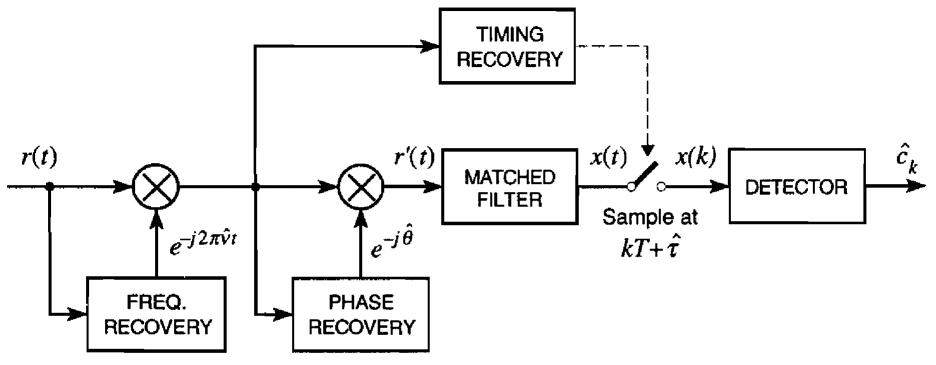
\includegraphics[width=0.8\columnwidth]{figs/example.png}
    \end{figure}
	\begin{itemize}
        \item Normalmente, a recuperação da portadora (fase e frequência) é feita antes da recuperação do tempo de símolo. Mas axistem diferentes arquiteturas que podem recuperar os parâmetros em outra ordem, inclusive em paralelo ou conjunta (\textit{joint estimation}).
    \end{itemize}
\end{frame}

\section{Estimador ML e MAP}

\begin{frame}
	\frametitle{Estimador ML e MAP}
	\begin{itemize}
		
		\item Existem basicamente dois critério amplamente empregados para a estimação de \(\hat{\boldsymbol{\lambdaup}}\): o criétio de máxima verossimilhança (ML) e o critério de máxima a posteriori (MAP), que originam os estimadores ML e MAP, respectivamente.
		
		\item Realizando a projeção de \(r(t)\) em um espaço de \(N\) funções ortonormais, obtemos, para o \(k\)-ésimo símbolo transmitido, o vetor \(\mathbf{r}_k \in \mathbb{R}^N\).
		
        \item Pelo o teorema de Bayes, tem-se a seguinte relação
        \begin{align}
            p(\hat{\boldsymbol{\lambdaup}}_k | \mathbf{r}_k) = \dfrac{p(\mathbf{r}_k \mid \hat{\boldsymbol{\lambdaup}}_k) p(\hat{\boldsymbol{\lambdaup}}_k)}{p(\mathbf{r}_k)}
        \end{align}

	\end{itemize}
\end{frame}

\begin{frame}[t]
    \frametitle{Estimador ML e MAP}

    \begin{itemize}
        \item \(p(\hat{\boldsymbol{\lambdaup}}_k)\) é a probabilidade a priori.
        \item \(p(\hat{\boldsymbol{\lambdaup}}_k | \mathbf{r}_k)\) é a probabilidade a posteriori.
        \item \(p(\mathbf{r}_k \mid \hat{\boldsymbol{\lambdaup}}_k)\) é a função de verossimilhança.
    \end{itemize}

    \begin{itemize}
        \item Como \(p(\mathbf{r}_k)\) é igual para \(\hat{\boldsymbol{\lambdaup}}_k\), podemos disconsidera-la.
        \item Quando a probabilidade a priori possui uma distribuição uniforme, também podemos disconsidera-la. Neste caso, o método MAP se torna igual ao ML
    \end{itemize}
\end{frame}

\section{Próxima aula}
\begin{frame}[t]
    \frametitle{Estimador ML e MAP}

    \begin{itemize}
        \item Derivação das equações de MAP e ML
        \item Apesentação de algumas arquiteturas de estimadores de fase.
    \end{itemize}
\end{frame}